\documentclass[a4paper,12pt]{article}
\usepackage[top = 2.5cm, bottom = 2.5cm, left = 2.5cm, right = 2.5cm]{geometry}
\usepackage[T1]{fontenc}
\usepackage[utf8]{inputenc}
\usepackage{multirow} 
\usepackage{booktabs} 
\usepackage{graphicx}
\usepackage[spanish]{babel}
\usepackage{setspace}
\setlength{\parindent}{0in}
\usepackage{float}
\usepackage{fancyhdr}
\usepackage{amsmath}
\usepackage{amssymb}
\usepackage{amsthm}
\usepackage[numbers]{natbib}
\newcommand\Mycite[1]{%
	\citeauthor{#1}~[\citeyear{#1}]}
\usepackage{graphicx}
\usepackage{subcaption}
\usepackage{booktabs}
\usepackage{etoolbox}
\usepackage{minibox}
\usepackage{hyperref}
\usepackage{xcolor}
\usepackage[skins]{tcolorbox}
%---------------------------

\newtcolorbox{cajita}[1][]{
	 #1
}

\newenvironment{sol}
{\renewcommand\qedsymbol{$\square$}\begin{proof}[\textbf{Solución.}]}
	{\end{proof}}

\newenvironment{dem}
{\renewcommand\qedsymbol{$\blacksquare$}\begin{proof}[\textbf{Demostración.}]}
	{\end{proof}}

\newtheorem{problema}{Problema}
\newtheorem{definicion}{Definición}
\newtheorem{ejemplo}{Ejemplo}
\newtheorem{teorema}{Teorema}
\newtheorem{corolario}{Corolario}[teorema]
\newtheorem{lema}[teorema]{Lema}
\newtheorem{prop}{Proposición}
\newtheorem*{nota}{\textbf{NOTA}}
\renewcommand\qedsymbol{$\blacksquare$}
\usepackage{svg}
\usepackage{pgfplots}
\pgfplotsset{compat=1.11}

\usepackage{tikz}
\usetikzlibrary{calc}

\usetikzlibrary{patterns}
\usepackage[framemethod=default]{mdframed}
\global\mdfdefinestyle{exampledefault}{%
linecolor=lightgray,linewidth=1pt,%
leftmargin=1cm,rightmargin=1cm,
}




\newenvironment{noter}[1]{%
\mdfsetup{%
frametitle={\tikz\node[fill=white,rectangle,inner sep=0pt,outer sep=0pt]{#1};},
frametitleaboveskip=-0.5\ht\strutbox,
frametitlealignment=\raggedright
}%
\begin{mdframed}[style=exampledefault]
}{\end{mdframed}}
\newcommand{\linea}{\noindent\rule{\textwidth}{3pt}}
\newcommand{\linita}{\noindent\rule{\textwidth}{1pt}}

\AtBeginEnvironment{align}{\setcounter{equation}{0}}
\pagestyle{fancy}

\fancyhf{}









%----------------------------------------------------------
\lhead{\footnotesize Geometría diferencial}
\rhead{\footnotesize  Rudik Roberto Rompich}
\cfoot{\footnotesize \thepage}


%--------------------------

\begin{document}
 \thispagestyle{empty} 
    \begin{tabular}{p{15.5cm}}
    \begin{tabbing}
    \textbf{Universidad del Valle de Guatemala} \\
    Departamento de Matemática\\
    Licenciatura en Matemática Aplicada\\\\
   \textbf{Estudiante:} Rudik Roberto Rompich\\
   \textbf{Correo:}  \href{mailto:rom19857@uvg.edu.gt}{rom19857@uvg.edu.gt}\\
   \textbf{Carné:} 19857
    \end{tabbing}
    \begin{center}
        Geometría diferencial - Catedrático: Alan Reyes\\
        \today
    \end{center}\\
    \hline
    \\
    \end{tabular} 
    \vspace*{0.3cm} 
    \begin{center} 
    {\Large \bf  Tarea
} 
        \vspace{2mm}
    \end{center}
    \vspace{0.4cm}
%--------------------------
\begin{problema}

    La región $1(\mathrm{z}<0)$ contiene un dieléctrico para el cual $\varepsilon_{r}=2.5$, mientras la región $2(\mathrm{z}>0)$ se caracteriza por un dieléctrico $\varepsilon_{r}=4$. Sea $\overrightarrow{E_{1}}=-30 \overrightarrow{a_{x}}+50 \overrightarrow{a_{y}}+70 \overrightarrow{a_{z}} \mathrm{~V} / \mathrm{m}$. Encontrar 
    \begin{enumerate}
        \item $\mathbf{D}_{2}$
        \begin{sol}
      Sea       
$$ D_{1}=\varepsilon\varepsilon_{r_1} E_{1}=\varepsilon_{0}(2.5)(-30,50,70)
$$

Ahora, tenemos: $D_{1n}-D_{2n}=\rho_{s}$ pero no hay carga en la superficie $\Rightarrow \rho_{s}=0$. $\Rightarrow \quad D_{1 n}=D_{2 n}, \text { como estamos en $z=0$ } \Rightarrow \quad D_{1 z}=D_{2 z} \Rightarrow \varepsilon_{0} \varepsilon_{r_{1}} E_{1 z}=\varepsilon_{0} \varepsilon_{r_{2}} E_{2 z}$

$$
\begin{aligned}
& \Rightarrow \quad E_{2 z}=\frac{\varepsilon_{0} \varepsilon_{r_{1}} E_{1 z}}{\varepsilon_{0} \varepsilon_{2 z}}=\frac{\varepsilon_{r_1}}{\varepsilon_{r_{2}}} \cdot E_{1 z}=\frac{2. 5}{4}(70)=\frac{\frac{5}{2}}{4}(70)  =\frac{5}{8}(70)=\frac{5}{4}(35)=\frac{175}{4} \frac{\mathrm{V}}{m}
\end{aligned}
$$

$\Rightarrow$ Para la componente tangencial, $E_{1 t}=E_{2 t}$ Tenemos $E_x$ y $E_y$:

$$
\begin{aligned}
& E_{2 x}=E_{1 x}=-30 \\
& E_{2 y}=E_{1 y}=50 \\
\Rightarrow E_{2}= & \left(-30,50, \frac{175}{4}\right) \mathrm{V} / \mathrm{m} \\
\Rightarrow D_{2}= & \varepsilon_{0} \varepsilon_{r 1} E_{2}=\varepsilon_{0}(4)\left(-30,50, \frac{175}{4}\right) \mathrm{V} / \mathrm{ms} \\
= & \varepsilon_{0}(-120,200,175) \mathrm{V} / \mathrm{m}
\end{aligned}
$$
        \end{sol}
        \item $\mathbf{E}_{2}$ 
        \begin{sol} Inciso anterior, $E_{2}=\left(-30,50, \frac{175}{4}\right) \mathrm{V} / \mathrm{m}$
        \end{sol}
        \item el ángulo entre $\mathbf{E}_{1}$ y la normal a la superficie.
        \begin{sol}
            Producto escalar $E_{1} \cdot \vec{a}_{z}=\left|E_{1}\right|\left|\vec{a}_{z}\right| \cos \theta$

            $$
            \begin{aligned}
            \Rightarrow \cos \theta & =\frac{E_{1} \cdot a_{z}}{\left|E_{1}\right|\left|a_{z}\right|}=\frac{70(1)}{\sqrt{(-30)^{2}+(50)^{2}+(70)^2}} \\
            & =\frac{70}{10 \sqrt{83}}=\frac{7}{\sqrt{83}} \\
            \Rightarrow \theta & =\operatorname{arcos}\left(\frac{7}{\sqrt{83}}\right)=39.79^{\circ}
            \end{aligned}
            $$
        \end{sol}
    \end{enumerate}
    
    

\end{problema}


\begin{problema}
Responda:
\begin{enumerate}
    \item Dado que $\vec{E}=-15 \overrightarrow{a_{x}}-8 \overrightarrow{a_{z}} \mathrm{~V} / \mathrm{m}$ en un punto de una superficie conductora, ¿cuál es la densidad de carga en la superficie en ese punto? Asuma que $\varepsilon=\varepsilon_{0}$.
    \begin{sol}
        $$
\begin{aligned}
& \Rightarrow D_{1 n}-D_{2 n}=\rho_{s} \Rightarrow D_{1 n}=\rho_{s} \\
& \Rightarrow \rho_{s}=D_{1 n}=\varepsilon E_{1 n}=\varepsilon_{0} E_{1} \cdot n=\varepsilon_0\left|E_{1}\right||n| \cos \theta
\end{aligned}
$$

$\Rightarrow$ No se nos da $n$ entonces solo podemos dejar expresada la ecuación

$$
\rho_{S}=\varepsilon_{0}\left(-15 a_{x}-8 a_{z}\right) \cdot n
$$
    \end{sol}
    \item La región $y \geq 2$ está ocupada por un conductor. Si la carga superficial del conductor es $20 \mathrm{nC} / \mathrm{m}^{2}$, encontrar $D$ afuera del conductor.
    \begin{sol}
        $$
\begin{aligned}
& \Rightarrow D_{1 n}-D_{2 n}=\rho_{s} \Rightarrow D_{1 n}=\rho_{1}, \Rightarrow D_{1 n}=\frac{20 n c}{m^{2}} \\
& \Rightarrow \vec{D}_{1}=D_{1 n} \vec{a}_{n}=\frac{20 n c}{m^{2}}(-\vec{a} y)=-20 \frac{nc}{m^2}\vec{a}_y
\end{aligned}
$$
    \end{sol}
\end{enumerate}


\end{problema}

\begin{problema}
    Una barra cilíndrica de carbono $\sigma=3 X 10^{4}$ tiene un radio de $5 \mathrm{~mm}$ y una longitud de $8 \mathrm{~cm}$. Si se mantiene a una diferencia de $9 \mathrm{~V}$. Encontrar:
    \begin{enumerate}
        \item la resistencia de la barra.
        \begin{sol}
            
$$
\begin{aligned}
R & =\rho\left(\frac{L}{A}\right)=\frac{1}{\sigma }\left(\frac{L}{\pi r^{2}}\right) = \frac{8 \times 10^{-2}}{\left(3 \times 10^{4}\right) \pi\left(5 \times 10^{-3}\right)^{2}} \\
& =\frac{8}{75 \pi}
\end{aligned}
$$
        \end{sol}
        \item  la corriente a través de la barra.
        \begin{sol}
            
$$
\Rightarrow V=I R \Rightarrow I=\frac{V}{R}=\frac{9}{8 / 75 \pi}=\frac{(75 \pi)(9)}{8}=\frac{675 \pi}{8}
$$
        \end{sol}
        \item  la potencia disipada por la barra.
        \begin{sol}
            $$
\begin{aligned}
P & =V I \Rightarrow P=(I R) I=I^{2} R=\left(\frac{675 \pi}{8}\right)^{2}\left(\frac{8}{75 \pi}\right) \\
& =\frac{6075 \pi}{8}
\end{aligned}
$$
        \end{sol}
    \end{enumerate}

\end{problema}

\begin{problema}
La densidad de corriente en un conductor cilíndrico de radio a está dada por:

$$
\vec{J}=10 e^{-\left(1-\frac{\rho}{a}\right)} \overrightarrow{a_{z}} \mathrm{~A} / \mathrm{m}^{2}
$$

Encontrar la corriente que pasa a través de la sección transversal del conductor.

\begin{sol}
    $$
\begin{aligned}
 I&=\oint_{s} J \cdot d s \\
& =\oint_{s} 10 e^{-(1-\rho / a)} \cdot \rho d \rho d \phi \\
& =\int_{0}^{2 \pi} \int_{0}^{a} 10 e^{-(1-\rho / a)} \cdot \rho d \rho d \phi \\
& =10 \int_{0}^{2 \pi} d \phi \int_{0}^{a} e^{-(1-\rho / a)} \cdot \rho d \rho\\
& =10(2 \pi)\left(\frac{a^{2}}{e}\right)=\frac{20 \pi a^{2}}{e}
\end{aligned}
$$
\end{sol}
\end{problema}

\begin{problema}
    Un alambre está hecho de cobre y consta de 150 vueltas. Si el radio de las vueltas es $6.5 \mathrm{~mm}$ y el diámetro del alambre es $0.4 \mathrm{~mm}$. Calcule la resistencia del alambre.
    \begin{sol}
        
$$
\begin{aligned}
\Rightarrow R & =\rho\left(\frac{L}{A}\right) \Rightarrow \rho=1.68 \times 10^{-8} \Omega m ; L=150\cdot 2\pi \cdot 6.5\times 10^{-3}; A =\pi r^{2}=\pi\left(\frac{0.4 \times 10^{-3}}{2}\right)^{2} \\
\Rightarrow R & =\left(1.68 \times 10^{-8} \Omega \mathrm{m}\right)\left(\frac{150 \cdot 2 \pi \cdot 6.5 \times 10^{-3}}{\pi\left(\frac{0.4 \times 10^{-3}}{2}\right)^{2}}\right)=0.819 \Omega
\end{aligned}
$$

    \end{sol}

\end{problema}

\begin{problema}
    Determinar el tiempo de relajación de:
    \begin{enumerate}
        \item Plástico duro $\left(\sigma=10^{-15} \mathrm{~S} / \mathrm{m}, \varepsilon=3.1 \varepsilon_{0}\right)$
        \begin{sol}
            
$$
\Rightarrow t=\frac{\varepsilon}{\sigma}=\frac{3.1 \varepsilon_{0}}{10^{-15} \frac{\mathrm{s}}{\mathrm{m}}}=2.741 \times 10^{4} \mathrm{~s} 
$$
        \end{sol}
        \item Mica $\left(\sigma=10^{-15} S / m, \varepsilon=6 \varepsilon_{0}\right)$
        \begin{sol}
            $$
t=\frac{\varepsilon}{\sigma}=\frac{6 \varepsilon_{0}}{10^{-15} \mathrm{~s} / \mathrm{m}}=5.305 \times 10^4 \mathrm{~s}
$$
        \end{sol}
        \item Agua destilada $\left(\sigma=10^{-4} S / m, \varepsilon=80 \varepsilon_{0}\right)$ 
        \begin{sol}
            $$
t=\frac{\varepsilon}{\sigma}=\frac{80 \varepsilon_{0}}{10^{-4} \mathrm{~s} / \mathrm{m}}=7.07 \times 10^{-6} \mathrm{~s}
$$
        \end{sol}
    \end{enumerate}


\end{problema}

\begin{problema}
    En la figura 33 la batería suministra 12 V. Considere $C_{1}=1.0 \mu \mathrm{F}, C_{2}=2.0 \mu \mathrm{F}, C_{3}=3.0 \mu \mathrm{F}$ y $C_{4}=4.0 \mu \mathrm{F}$.
    \begin{figure}[H]
        \centering
        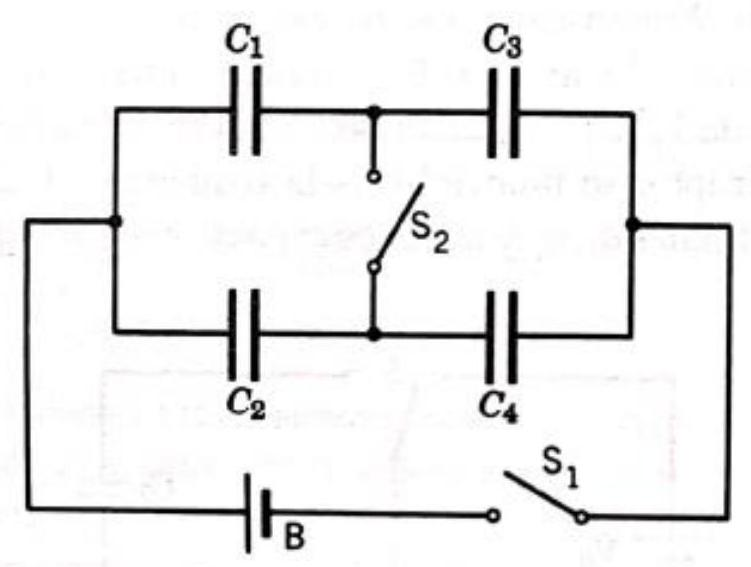
\includegraphics[scale=0.3]{imagenes/1.jpg}
    \end{figure}
    \begin{enumerate}
        \item Halle la carga sobre cada capacitor cuando el intertuptor $S_{1}$ se cierra 
        \begin{sol}En serie:
            $$
\begin{aligned}
\Rightarrow  \frac{1}{C_{13}} & =\frac{1}{C_{1}}+\frac{1}{C_{3}} \\
& =\frac{1}{1.0 \mu}+\frac{1}{3.0 \mu}
\end{aligned}
$$


Además, $V_{1,3}=V_{2,4}=V$: 

$$
\begin{aligned}
& \Rightarrow Q_{1,3}=C_{1,3} V_{1,3}=\left(\frac{1}{\frac{1}{1.0 \mu}+\frac{1}{3.0\mu}}\right)(12)= 9\mu \\
& \Rightarrow Q_{13}=Q_{1}=Q_{2}= 9\mu 
\end{aligned}
$$
En serie:
$$
\begin{aligned}
&\Rightarrow  \frac{1}{C_{24}}=\frac{1}{C_{2}}+\frac{1}{C_{4}}=\frac{1}{2.0 \mu}+\frac{1}{4.0 \mu} \\
& \Rightarrow C_{24}=\frac{1}{\frac{1}{2.0 \mu}+\frac{1}{4.0 \mu}} \\
& \Rightarrow Q_{24}=C_{24} V_{24}=\left(\frac{1}{\frac{1}{2.0 \mu}+\frac{1}{4.0 \mu}}\right)(12)= 1.6\times 10^{-5}\\
& \Rightarrow Q_{24}=Q_{2}=Q_{4}=1.6\times 10^{-5}
\end{aligned}
$$
        \end{sol}
        \item Cuando (más tarde) el interruptor $\mathrm{S}_{2}$ también se cierra. Considere $C_{1}=1.0 \mu \mathrm{F}, C_{2}=2.0 \mu \mathrm{F}, C_{3}=3.0 \mu \mathrm{F}$ y $C_{4}=4.0 \mu \mathrm{F}$.
        \begin{sol}
            $$
\begin{aligned}
C_{12} & =C_{1}+C_{2}=1.0 \mu+2.0 \mu=3.0 \mu \\
C_{34} & =C_{3}+C_{4}=3.0\mu+4.0\mu=7.0 \mu \\
\Rightarrow C_{T} & =\frac{1}{C_{12}}+\frac{1}{C_{34}}=\frac{1}{3.0 \mu}+\frac{1}{7.0 \mu}\\
\Rightarrow Q_{12} & =Q_{34}=Q_{T}=\left(\frac{1}{3.0 \mu}+\frac{1}{7.0 \mu}\right)(12)
\end{aligned}
$$


\begin{align*}
    V_{12} &= \frac{Q_{12}}{C_{12}} = 1.905\times 10^{12}\implies V_{12}=V_1=V_2\\
    V_{34} &= \frac{Q_{34}}{C_{34}} = 8.163\times 10^{11}\implies V_{34}=V_3=V_4
\end{align*}
Entonces: 
\begin{align*}
    Q_1 &= C_1V_1=1.905\mu \\
    Q_2 &= C_2V_2=3.81\mu\\
    Q_3 &= C_3V_3=2.449\mu\\
    Q_4 &= C_4V_4=3.265\mu\\
\end{align*}
        \end{sol}
    \end{enumerate}
    
\end{problema}

\begin{problema}
    Halle la capacitancia equivalente entre los puntos $x$ y $y$ en la figura 34. Suponga que $C_{2}=10 \mu \mathrm{F}$ y que los otros capacitores son todos de $4.0 \mu \mathrm{F}$. (Sugerencia: Aplique una diferencia de potencial $V$ entre $x$ y $y$, y escriba todas las relaciones que contengan a las cargas y las diferencias de potencial en cada uno de los capacitores.)
    \begin{figure}[H]
        \centering
        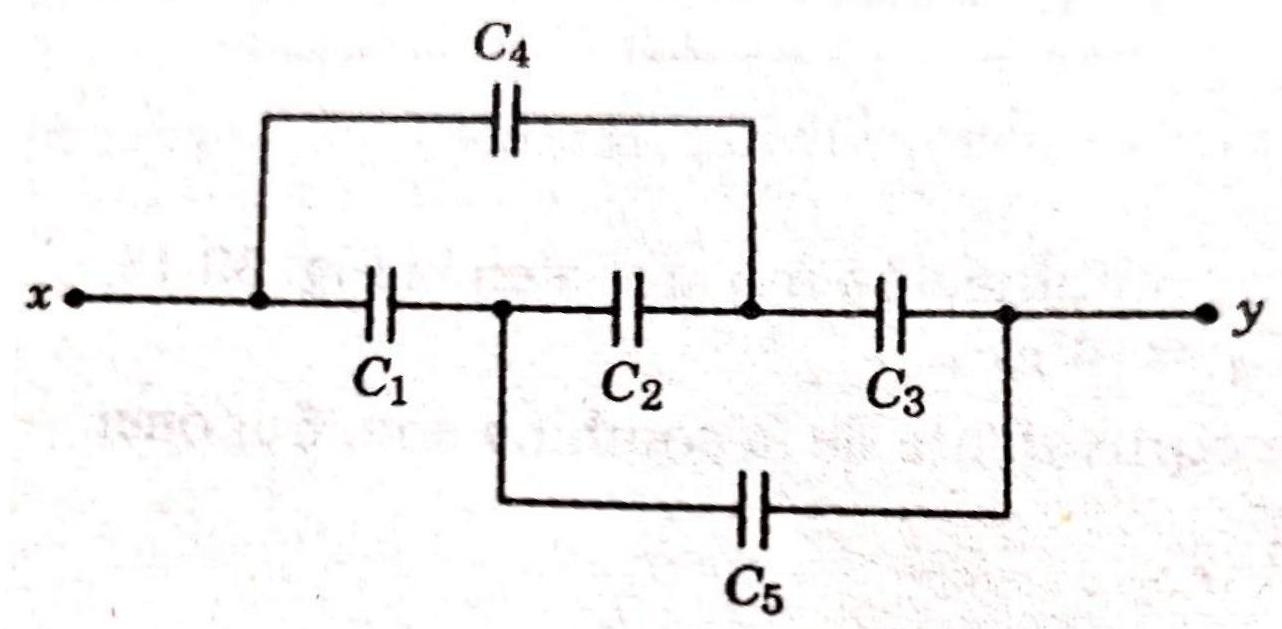
\includegraphics[scale=0.3]{imagenes/2.jpg}
    \end{figure}
    \begin{sol}
        Sea 
        $$C_1=C_3=C_4=C_5=4.0\mu F; C_2=10\mu F $$
        Sea 
        $$\frac{C_1}{C_3}=\frac{C_4}{C_5}=1$$
        \begin{align*}
            \frac{1}{C_{14}} &= \frac{1}{C_1}+\frac{1}{C_4} = \frac{1}{4.0\mu}+\frac{1}{4.0\mu}\implies C_{14} = 2.0\mu\\
            \frac{1}{C_{35}} &= \frac{1}{C_3}+\frac{1}{C_5} = \frac{1}{4.0\mu}+\frac{1}{4.0\mu}\implies C_{45} = 2.0\mu\\
        \end{align*}
        $$C_T= C_{14}+C_{34}=4\mu$$
    \end{sol}
\end{problema}

\begin{problema}
    Responda: 
    \begin{enumerate}
        \item Tres capacitores están conectados en paralelo. Cada uno tiene un área de placa $A$ y un espaciamiento entre placas $d$. ¿Cuál debe ser el espaciamiento de un solo capacitor de área de placa $A$ si su capacitancia es igual a la de la combinación en paralelo? 
        \begin{sol}
            Sea $C=\frac{\varepsilon_{0} A}{d}$
            $$ C_{T}=C_{1}+C_{2}+C_{3}=3 C_{0}=\frac{3 \varepsilon_{0} A}{d}$$
Entonces 
$$\Rightarrow C_{T}=\frac{3 \varepsilon_{0} A}{d} \Rightarrow \frac{\varepsilon_{0} A}{d^{\prime}}=\frac{3 \varepsilon_{0} A}{d}$$


$$\Rightarrow \frac{1}{d^{\prime}}=\frac{3}{d} \Rightarrow d^{\prime}=\frac{d}{3}$$
        \end{sol}
        \item ¿Cuál debe ser el espaciamiento cuando los tres capacitores están conectados en serie?
        \begin{sol}
            $$
\begin{aligned}
& \frac{1}{C_{T}}=\frac{1}{C_{1}}+\frac{1}{C_{2}}+\frac{1}{C_{2}} \Rightarrow \frac{1}{C_{T}}=3\left(\frac{1}{C_{0}}\right) \\
\Rightarrow & C_{T}=\frac{C_{0}}{3} \Rightarrow \frac{\varepsilon_{0} A}{d^{\prime \prime}}=\frac{C_{0}}{3} \\
\Rightarrow & \frac{\varepsilon_{0} A}{d^{\prime \prime}}=\frac{\left(\frac{\varepsilon_{0} A}{d}\right)}{3} \Rightarrow \frac{\varepsilon_{0} A}{d^{\prime \prime}}=\frac{\varepsilon_{0} A}{3 d} \\
\Rightarrow & \frac{1}{d^{\prime \prime}}=\frac{1}{3 d} \Rightarrow d^{\prime \prime}=3 d
\end{aligned}
$$
        \end{sol}
    \end{enumerate}


\end{problema}

\begin{problema}
    Sea una cascarón esférico dieléctrico, tal que $\varepsilon=\varepsilon_{0} \varepsilon_{r}$, para a $<r<b$ y $\varepsilon=\varepsilon_{0}$ para $0<r<a$. Si se coloca una carga $Q$ en el centro del cascarón, encuentre:
    \begin{enumerate}
        \item $\mathbf{P}$ para $\mathbf{a}<\mathbf{r}<b$
        \begin{sol}
            Para encontrar la polarización $\mathbf{P}$ en la región dieléctrica ($a<r<b$). Usamos la ley de Gauss:
            $$\oint \mathbf{D} \cdot d\mathbf{A} = Q_{enc}$$
            Considerando que $\mathbf{D} = \varepsilon \mathbf{E}$, tenemos:

$$D_r \oint dA = Q_{enc}\implies D_r (4\pi r^2) = Q_{enc}\implies D_r = \frac{Q_{enc}}{4\pi r^2}$$

Para $a<r<b$, $\varepsilon = \varepsilon_0 \varepsilon_r$, entonces:

$$\varepsilon_0 \varepsilon_r E_r = \frac{Q_{enc}}{4\pi r^2}\implies E_r = \frac{Q_{enc}}{4\pi \varepsilon_0 \varepsilon_r r^2}$$

La relación entre $\mathbf{P}$ y $\mathbf{E}$ es: 

$$\mathbf{P} = \chi_e \varepsilon_0 \mathbf{E}$$

En donde, $\varepsilon_r = 1 + \chi_e$, tal que: 

$$\mathbf{P} = (\varepsilon_r - 1) \varepsilon_0 \mathbf{E}= \varepsilon_0 (\varepsilon_r - 1) \frac{Q_{enc}}{4\pi \varepsilon_0 \varepsilon_r r^2} \hat{\mathbf{r}}=  (\varepsilon_r - 1) \frac{Q_{enc}}{4\pi\varepsilon_r r^2} \hat{\mathbf{r}}$$

        \end{sol}
        \item $\rho_{\rho v}$, para $a<r<b$
        \begin{sol}
            Sea
            \begin{align*}
                \nabla \cdot \mathbf{P} &= -\rho_v\\
                \frac{1}{r^2} \frac{\partial}{\partial r}(r^2 P_r) &= -\rho_v\\
                \frac{1}{r^2} \frac{\partial}{\partial r} \left( r^2 \frac{(\varepsilon_r - 1)Q_{enc}}{4\pi \varepsilon_r r^2} \right) &= -\rho_v\\
                -\frac{1}{r^2} \frac{\partial}{\partial r} \left( \frac{(\varepsilon_r - 1)Q_{enc}}{4\pi \varepsilon_r} \right) &= \rho_v\\
                0 &= \rho_v
            \end{align*}

        \end{sol}
        \item $\rho_{\rho s}$ en $r=a$ y $r=b$
        \begin{sol}
            Consideramos los dos casos: 
            \begin{enumerate}
                \item Consideremos primero $r = a$:
                $$\rho_s(a) = \mathbf{P}(a^+) \cdot \hat{\mathbf{r}} - \mathbf{P}(a^-) \cdot \hat{\mathbf{r}}$$
                Para $r<a$, $\mathbf{P} = \mathbf{0}$ (ya que no hay polarización en el espacio vacío), y para $r>a$, usamos la expresión obtenida en la parte 1):

                $$\rho_s(a) = \frac{(\varepsilon_r - 1)Q_{enc}}{4\pi \varepsilon_r a^2}$$
                \item Tenemos $r = b$:

                $$\rho_s(b) = \mathbf{P}(b^-) \cdot \hat{\mathbf{r}} - \mathbf{P}(b^+) \cdot \hat{\mathbf{r}}$$
                
                Para $r>b$, $\mathbf{P} = \mathbf{0}$ (ya que no hay polarización en el espacio vacío), y para $r<b$, usamos la expresión obtenida en la parte 1):
                
                $$\rho_s(b) = -\frac{(\varepsilon_r - 1)Q_{enc}}{4\pi \varepsilon_r b^2}$$
            \end{enumerate}
            


        \end{sol}
    \end{enumerate}

\end{problema}

\begin{problema}
    El capacitor de placas paralelas tiene una cuarta parte que es llenada con mica $\left(\epsilon_{r}=6\right)$. Encuentre la capacitancia.
\begin{figure}[H]
    \centering
    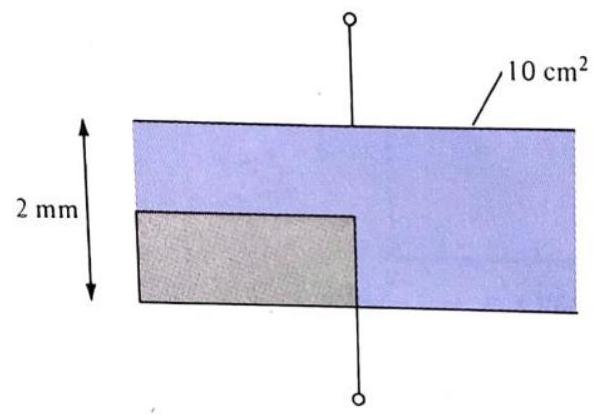
\includegraphics[scale=0.3]{imagenes/3.jpg}
\end{figure}
\begin{sol}
    Para resolver este problema, consideramos la siguiente estructura: 
    \begin{figure}[H]
        \centering 


\tikzset{every picture/.style={line width=0.75pt}} %set default line width to 0.75pt        

\begin{tikzpicture}[x=0.75pt,y=0.75pt,yscale=-1,xscale=1]
%uncomment if require: \path (0,300); %set diagram left start at 0, and has height of 300

%Shape: Capacitor [id:dp1791853626103529] 
\draw   (282.15,150) -- (282.02,114) (261.98,106.08) -- (301.98,105.92) (262.02,114.08) -- (302.02,113.92) (281.98,106) -- (281.85,70) ;
%Shape: Capacitor [id:dp13531026535353918] 
\draw   (282.46,230) -- (282.32,194) (262.29,186.08) -- (302.29,185.92) (262.32,194.08) -- (302.32,193.92) (282.29,186) -- (282.15,150) ;
%Shape: Capacitor [id:dp6484268321795906] 
\draw   (415.15,184) -- (415.02,148) (394.98,140.08) -- (434.98,139.92) (395.02,148.08) -- (435.02,147.92) (414.98,140) -- (414.85,104) ;
%Straight Lines [id:da14198580624174784] 
\draw    (229,71.2) -- (457,71.2) ;
%Straight Lines [id:da1563691602950098] 
\draw    (230,228.2) -- (458,228.2) ;
%Straight Lines [id:da6538337657012104] 
\draw    (230,228.2) -- (229,71.2) ;
%Straight Lines [id:da020143135859299166] 
\draw    (458,228.2) -- (457,71.2) ;
%Straight Lines [id:da4098651295245336] 
\draw    (415.52,226.5) -- (414.52,69.5) ;
%Straight Lines [id:da9576054481622913] 
\draw [color={rgb, 255:red, 144; green, 19; blue, 254 }  ,draw opacity=1 ] [dash pattern={on 4.5pt off 4.5pt}]  (229.5,149.7) -- (348,149.2) ;
%Straight Lines [id:da8178166159938771] 
\draw [color={rgb, 255:red, 144; green, 19; blue, 254 }  ,draw opacity=1 ] [dash pattern={on 4.5pt off 4.5pt}]  (348,149.2) -- (349,227.2) ;
%Straight Lines [id:da5747579381861089] 
\draw [color={rgb, 255:red, 144; green, 19; blue, 254 }  ,draw opacity=1 ]   (195,176.2) -- (245,176.97) ;
\draw [shift={(247,177)}, rotate = 180.88] [color={rgb, 255:red, 144; green, 19; blue, 254 }  ,draw opacity=1 ][line width=0.75]    (10.93,-3.29) .. controls (6.95,-1.4) and (3.31,-0.3) .. (0,0) .. controls (3.31,0.3) and (6.95,1.4) .. (10.93,3.29)   ;

% Text Node
\draw (159,173) node [anchor=north west][inner sep=0.75pt]  [color={rgb, 255:red, 144; green, 19; blue, 254 }  ,opacity=1 ] [align=left] {mica};
% Text Node
\draw (309,180.4) node [anchor=north west][inner sep=0.75pt]    {$C_{1}$};
% Text Node
\draw (309,100.4) node [anchor=north west][inner sep=0.75pt]    {$C_{3}$};
% Text Node
\draw (373,134.4) node [anchor=north west][inner sep=0.75pt]    {$C_{2}$};


\end{tikzpicture}
    \end{figure}
    Tenemos: 

    \begin{enumerate}
        \item Para $C_1$: 
        $$C_1 = \frac{(\varepsilon_{mica} * (A/2))}{d/2} =\frac{(6)(\varepsilon_0) * (A/2)}{d/2}=\frac{(6)(\varepsilon_0) * (A)}{d}$$
        \item Para $C_2$: 
        $$C_2 = \frac{(\varepsilon_{aire} * (A/2))}{d/2} =\frac{(1)(\varepsilon_0) * (A/2)}{d}=\frac{(\varepsilon_0) * (A/2)}{d}$$
        \item Para $C_3$:
        $$C_3 = \frac{(\varepsilon_{aire} * (A/2))}{d/2} =\frac{(1)(\varepsilon_0) * (A/2)}{d/2}=\frac{(\varepsilon_0) * (A)}{d}$$
    \end{enumerate}
    
    Ahora, combinamos las capacitancias. Primero, encontramos la capacitancia equivalente de la combinación en serie de $C_1$ y $C_3$:

$$\frac{1}{C_{13}} = \frac{1}{ C_1} + \frac{1}{C_3} = \frac{d}{6\varepsilon_0 A}+\frac{d}{\varepsilon_0A}=\frac{7d}{6\varepsilon_0A}$$

Luego, sumamos $C_{13}$ y $C_2$ en paralelo para obtener la capacitancia total:

$$C_{T} = C_{13} + C_2= \frac{6\varepsilon_0A}{7d }+\frac{(\varepsilon_0)A}{2d}=\frac{\varepsilon_0 A}{d}\left(\frac{6}{7}+\frac{1}{2}\right)= \frac{\varepsilon_0(10\times 10^{-2})}{2\times 10^{-3}} \frac{19}{14}=\frac{475}{7}\varepsilon_0 $$



\end{sol}
\end{problema}

\begin{problema}
    Para un medio anisotrópico

$$
\left[\begin{array}{l}
D_{x} \\
D_{y} \\
D_{z}
\end{array}\right]=\epsilon_{0}\left[\begin{array}{lll}
5 & 1 & 1 \\
1 & 5 & 1 \\
1 & 1 & 5
\end{array}\right]\left[\begin{array}{l}
E_{x} \\
E_{y} \\
E_{z}
\end{array}\right]
$$

Obtener: 

\begin{enumerate}
    \item $\vec{E}=15 \overrightarrow{a_{x}}-10 \overrightarrow{a_{y}} V / m$
    \begin{sol}

        \begin{align*}
            \left[\begin{array}{l}
                D_{x} \\
                D_{y} \\
                D_{z}
                \end{array}\right]&=\epsilon_{0}\left[\begin{array}{lll}
                5 & 1 & 1 \\
                1 & 5 & 1 \\
                1 & 1 & 5
                \end{array}\right]\left[\begin{array}{l}
                15\\
                -10 \\
                0
                \end{array}\right]\\
                &=\epsilon_{0} \left[\begin{array}{l}
                    65\\
                    -35\\
                    5
                    \end{array}\right]
        \end{align*}
    \end{sol}
    \item $\vec{E}=15 \overrightarrow{a_{x}}+230 \overrightarrow{a_{y}}-20 \overrightarrow{a_{z}} V / m$
    \begin{sol}
        \begin{align*}
            \left[\begin{array}{l}
                D_{x} \\
                D_{y} \\
                D_{z}
                \end{array}\right]&=\epsilon_{0}\left[\begin{array}{lll}
                5 & 1 & 1 \\
                1 & 5 & 1 \\
                1 & 1 & 5
                \end{array}\right]\left[\begin{array}{l}
                15\\
                230 \\
                -20
                \end{array}\right]\\
                &=\epsilon_{0} \left[\begin{array}{l}
                    285\\
                    1145\\
                    145
                    \end{array}\right]
        \end{align*}
        
        
    \end{sol}
\end{enumerate}

\end{problema}


%---------------------------
%\bibliographystyle{apa}
%\bibliography{referencias.bib}

\end{document}